\documentclass{article}
\usepackage{amsmath}
\usepackage{fancyhdr}
\usepackage{geometry}
\usepackage{amssymb}
\usepackage{graphicx}
\usepackage{subfigure}
\usepackage{listings}

\lstset{
    language=R,
    basicstyle=\ttfamily\footnotesize,
    captionpos=b
}

% Page margins
\geometry{a4paper, margin=1in}

% Define header
\pagestyle{fancy}
\fancyhf{}
\fancyhead[L]{Student Number: 1462539}
\fancyhead[C]{MAST20005}
\fancyhead[R]{\thepage}

\title{Assignment 1}
\author{}
\date{}

\begin{document}

% Title page
\begin{titlepage}
    \centering
    \vspace*{2in}
    {\Huge \textbf{Assignment 1}}\\[1.5cm]
    {\Large MAST20005: Statistics}\\[0.5cm]
    {\Large Kevin Yu}\\[0.5cm]
    {\Large Student Number: 1462539}\\[2in]
    \vfill
    \large \textbf{\today}
    \vfill
\end{titlepage}

\newpage
\section*{Exercise 1}
\begin{figure}[h!]
    \centering
    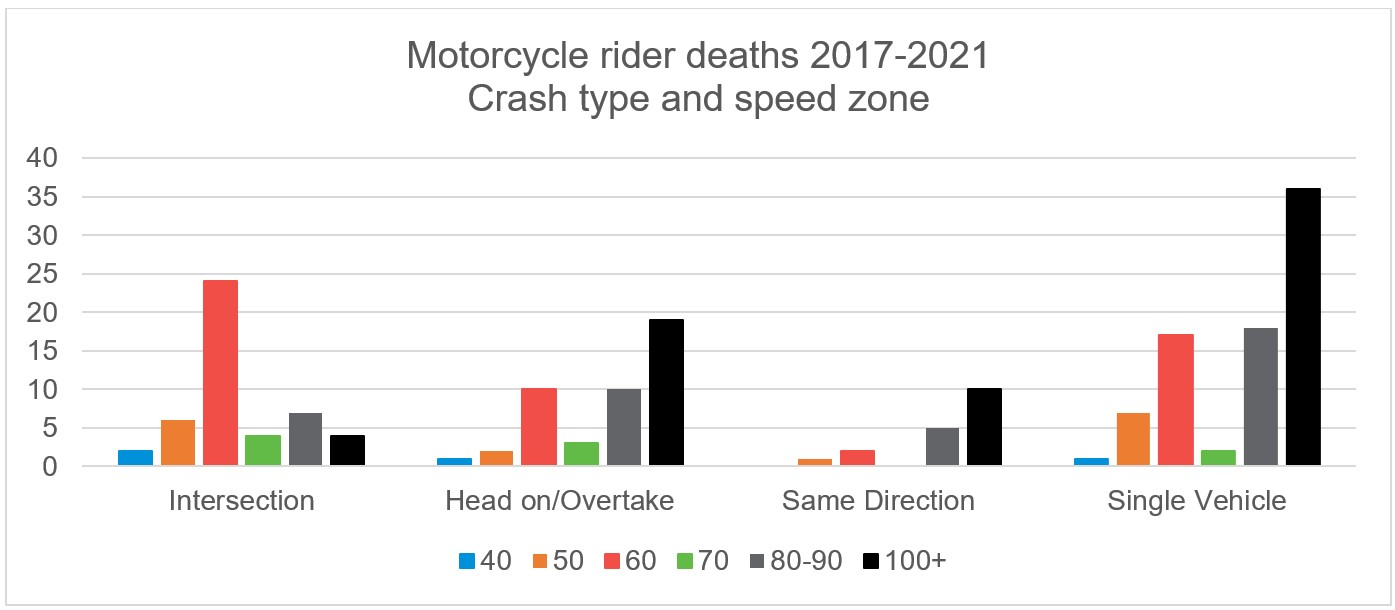
\includegraphics[width=0.8\textwidth]{images/motorcycle-rider-deaths.jpg}
    \caption{Motorcycle Rider Deaths 2017-2021 from TAC}
    \label{fig:motorcycle-deaths}
\end{figure}

\subsection*{Part 1}
The above graph represents the number of motorcycle rider deaths in Victoria from 2017 to 2021, retrieved from the Transport Accident Commission (TAC) website \footnote[1]{https://www.tac.vic.gov.au/road-safety/statistics/summaries/motorcycle-crash-data}. Its purpose is to provide a visual representation to inform riders on the danger of riding motorcycles and to encourage them to take necessary precautions to reduce the number of deaths. Precautions can include placing yourself where you can see and be seen in intersections, appropriate Crash Avoidance Space, and maintaining a safe speed. \\

\subsection*{Part 2}
\begin{itemize}
    \item The data is shown clearly, with distinct colour-coded bars and its respective legend representing different speed zones across various crash types. The title is concise and informative, and there are no unnecessary distractions in the graph.
    \item The graph uses a common scale (y-axis) for comparing number of deaths acorss different crash type, which makes us easier to compare. This directly contrasts the still birthrate graph presented in the lecture, where it used different scales for domiciliary and overall deliveries, making it difficult to compare the two. Furthermore, the alingment is uniform and consistent, making it easier to read and interpret the data. Lastly, they have used a bar graph, which is a great choice for comparing data across different categories.
    \item The graph is flat, with no 3D effects or shadows that may distort the data; while also containing all the necessary information to successfully convey the message to the audience. The graph may be improved by encorporating patterns to the bar, which would make it more accessible to individuals with colour blindness.
    \item The graph has good visual encoding with each color representing a specific speed zone, and the height of the bars representing the number of deaths. The legend is placed at the bottom of the graph, which is a good location as it does not obstruct the data.
    \item This graph uses one of the standard form of visualisation, a bar chart, which is a good choice for comparing data across different categories (in this case, crash type). $\quad \blacksquare$
\end{itemize}


\newpage
\section*{Exercise 2}

\subsection*{Part 1}

$\text{Please note that I have abbreviated } \sum_{i=1}^m \text{ as } \sum \text{ at some places to avoid overcrowding}$

$$
\begin{aligned}
L(\sqrt{ p }) &= \prod_{i=1}^{m} \binom{n}{x_{i}} (\sqrt{ p })^{x_{i}}(1-\sqrt{ p })^{n-x_{i}} \\
&= \prod_{i=1}^m \left[ \binom{n}{x_{i}}\right] (\sqrt{ p })^{\sum x_{i}}(1-\sqrt{ p })^{\sum (n-x_{i})} \\
\implies \ln{L(\sqrt{ p })} &= \ln{\prod_{i=1}^m \left[ \binom{n}{x_{i}}\right]} + \sum_{i=1}^m{(x_i)}\ln{\sqrt{ p }}+\sum_{i=1}^m{(n-x_{i})}\ln{(1-\sqrt{p})} \\
\implies \frac{d}{d\sqrt{ p }}[\ln{L(\sqrt{ p })})] &= \frac{\sum x_{i} \cdot \frac{1}{2} p^{1/2}}{\sqrt{ p }} + \frac{\left( mn - \sum x_{i} \right) \cdot -\frac{1}{2} p^{1/2}}{1 - \sqrt{ p }} \\
&= \frac{(1-\sqrt{ p })p^{-1/2} \sum x_{i} - mn + \sum x_{i}}{2\sqrt{ p } (1-\sqrt{ p })}
\end{aligned}
$$

$\text{Setting } \frac{d}{d\sqrt{ p }}[\ln{L(\sqrt{ p })})]  = 0 \text{ yields,}$

$$
\begin{aligned}
&(1-\sqrt{ p })p^{-1/2} \sum_{i=1}^m x_{i} - mn + \sum_{i=1}^m x_{i} = 0 \\
\implies &(p^{-1/2} - 1) \sum_{i=1}^m x_{i} - mn + \sum_{i=1}^m x_{i} = 0 \\
\implies &p^{-1/2} \sum_{i=1}^m x_{i} - mn = 0 \\
\implies &p^{-1/2} = \frac{mn}{\sum x_{i}} = \frac{n}{\bar{X}_{m}} \\
\implies &p^{1/2} = \frac{\bar{X}_{m}}{n} \\
& \therefore p = \frac{\bar{X}_{m}^2}{n^2} \qquad \blacksquare
\end{aligned}
$$

\subsection*{Part 2}
$$
\begin{aligned}
\bar{x}_{3} &= \frac{1}{3} (1 + 3 + 3) = \frac{7}{3} \\
\therefore p &= \frac{(7/3)^2}{5^2} = \frac{49}{9 \cdot 25} = \frac{49}{225} = 0.21\dot{7} \qquad \blacksquare
\end{aligned}
$$


\newpage
\section*{Exercise 3}

\subsection*{Part 1}

$$
\begin{aligned}
\mu(\theta) &= \int_{1}^\infty x \theta \left( \frac{1}{\theta} \right)^{\theta + 1} \, dx \\
&= \theta \int _{1}^\infty x^{-\theta} \, dx \\
&= \theta \cdot \frac{1}{\theta - 1} = \frac{\theta}{\theta - 1}
\end{aligned}
$$

now let $\mu(\theta) = \bar{X}$,

$$
\begin{aligned}
\implies &\frac{\theta}{\theta - 1} = \bar{X} \\
\implies & \theta = \bar{X}\theta - \bar{X} \\
\implies &\theta(1-\bar{X}) = -\bar{X} \\
\therefore \hat{\Theta}_{MM} &= \frac{\bar{X}}{\bar{X} - 1} \qquad \blacksquare
\end{aligned}
$$

\newpage
\subsection*{Part 2}

In addition to the variance, we can calculate
\begin{itemize}
    \item the range (max - min) to measure the spread of the data,
    \item the interquartile range (IQR), the difference between the third and first quartiles, which is less sensitive to outliers,
    \item the median as a measure of central tendency that is less sensitive to outliers.
\end{itemize}

Now, let $y_{(1)}, y_{(2)}, \dots, y_{(9)}$ and $z_{(1)}, z_{(2)}, \dots, z_{(9)}$ be the ordered samples from Sample 1, Sample 2 respectively. \\

For Sample 1, $y_{(1)} = 1.333$ and $y_{(9)} = 1.684$ so the range is $1.684 - 1.333 = 0.351$.  \\ 

For Sample 2, $z_{(1)} = 1.333$ and $z_{(9)} = 1.523$ so the range is $1.523 - 1.333 = 0.190$.  \\

Now to calculate the interquantile range, we recall from the lecture that having $x_{(1)}, x_{(2)}, \dots, x_{(n)}$ as the ordered observations; let the $p$-th quantile of the observations be denoted by $\hat{c}_p$ where $0 < p < 1$. Then, letting $k = 1 + (n-1)p$ and $t$ and $w$ be the whole and fractional part of $k$ respectively, (i.e. $t = \lfloor k \rfloor$ and $w = k - t$),

$$
\hat{c}_p = x_{(t)} + w(x_{(t+1)} - x_{(t)}).
$$
\\
Therefore, for Sample 1, the first quartile ``position'' is at $1 + (9-1)(0.25) = 3$ so the first quartile is $\hat{q}_1 = \hat{c}_{0.25} = y_{(3)} = 1.447$. The third quartile "position" is at $1 + (9-1)(0.75) = 7$ so the third quartile is $y_{(7)} = 1.577$. Hence, the IQR is $1.577 - 1.447 = 0.130$. \\

For Sample 2, the first and third quartile ``position'' is the same as Sample 1. Therefore, the first quartile is $z_{(3)} = 1.333$ and the third quartile is $z_{(7)} = 1.333$. Hence, the IQR is $1.333 - 1.333 = 0$. We also note that since IQR of Sample 2 is 0, so $z_{(9)} = 1.523$ is an extreme outlier. \\

Finally, the median of Sample 1 is $y_{(5)} = 1.529$ and the median of Sample 2 is $z_{(5)} = 1.333$. \\

Ultimately, the range and IQR of Sample 1 are greater than those of Sample 2. This suggests that Sample 1 has a greater variability, while Sample 2 has the same value for the first, second (medium) and third quartiles, indicating that the data is more concentrated around a single value. $\blacksquare$

\begin{figure}[h!]
    \centering
    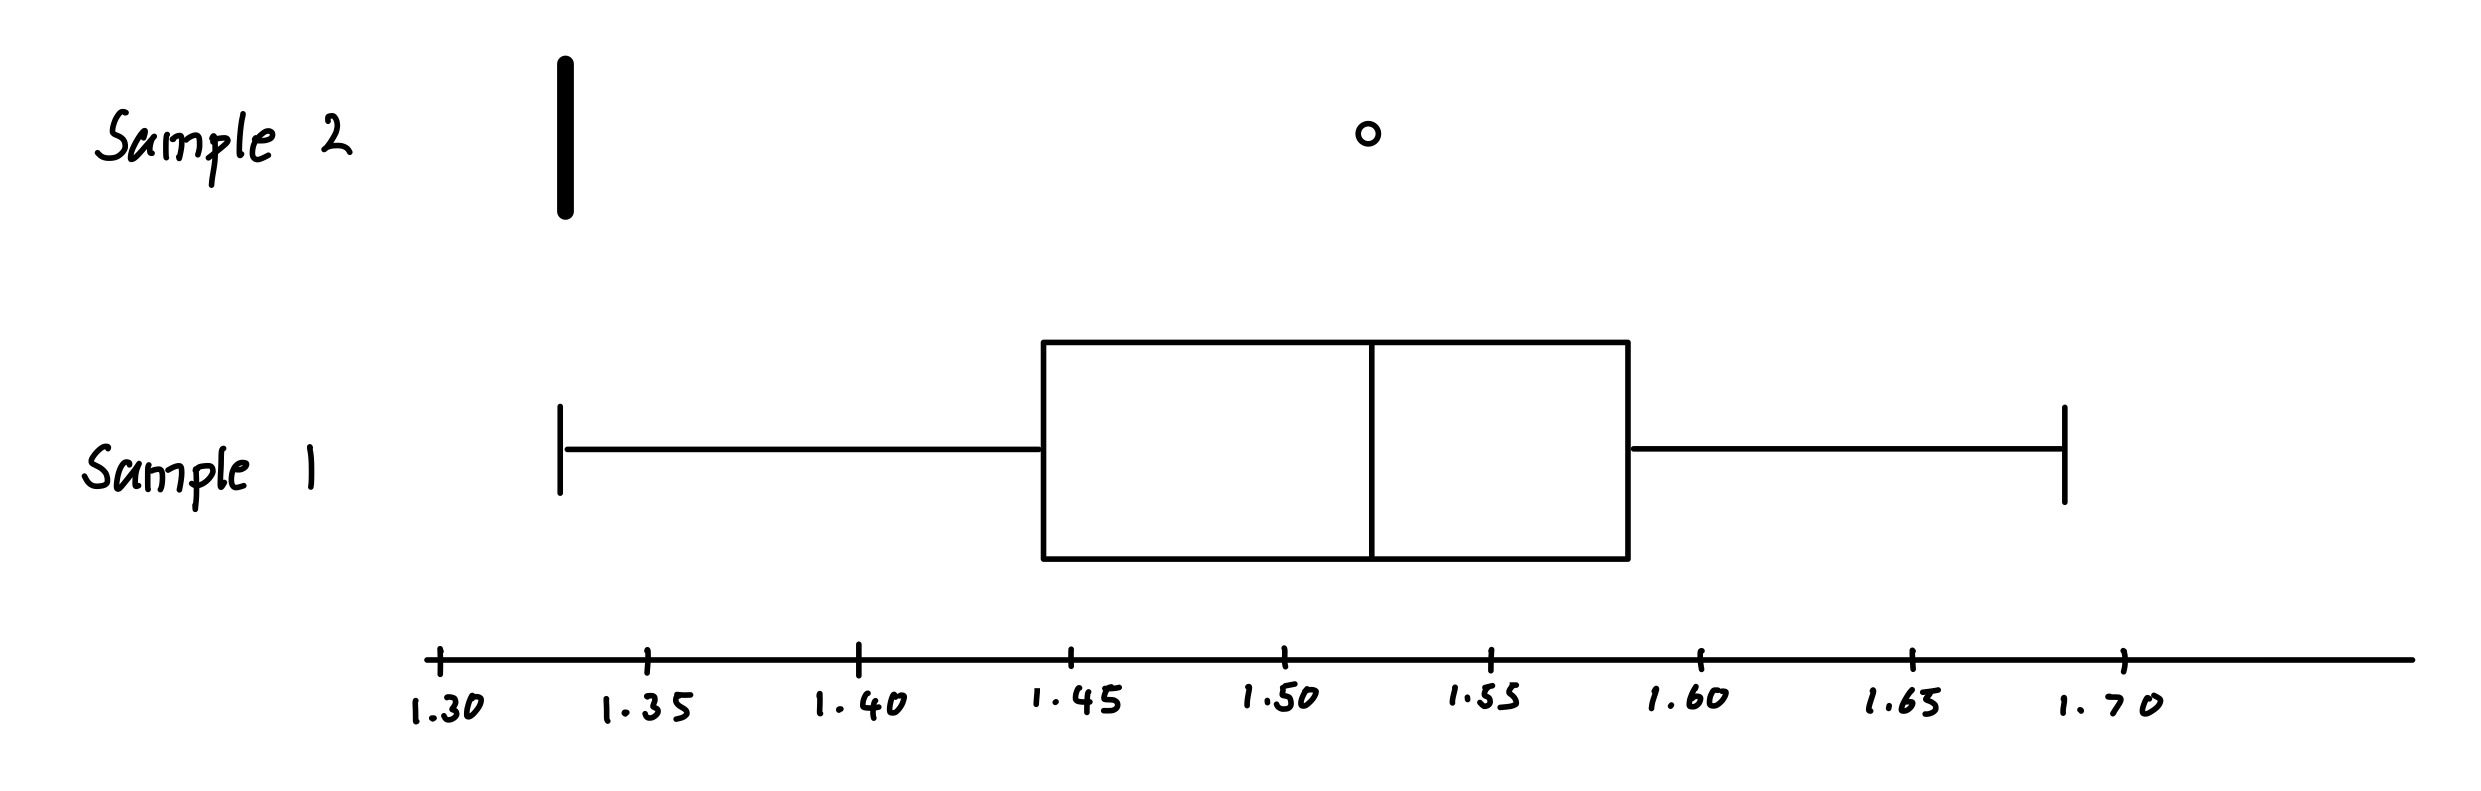
\includegraphics[width=0.8\textwidth]{images/boxplot.jpg}
    \caption{Boxplot of Sample 1 and Sample 2}
    \label{fig:boxplot}
\end{figure}

\newpage
\section*{Exercise 4}

\subsection*{Part 1}

\textit{Unbiasedness:} An estimator $T$ is unbiased for $\mu$ if $\mathbb{E}(T) = \mu$.

\begin{itemize}
    \item \textbf{For $T_1$:}
    $$
    \mathbb{E}(T_1) = \mathbb{E}\left(\frac{1}{6} \sum_{i=1}^{6} X_i\right) = \frac{1}{6} \sum_{i=1}^{6} \mathbb{E}(X_i) = \frac{1}{6} \times 6\mu = \mu
    $$
    So, $T_1$ is an unbiased estimator of $\mu$.

    \item \textbf{For $T_2$:}
    Following the same steps as above, $T_2$ is also an unbiased estimator of \( \mu \) \\
    (since $X_i, \; Y_i \sim_{i.i.d.} N(\mu, \sigma^2 = 25 \, \text{km/h}^2)$).

    \item \textbf{For $T_3$:}
    $$
    \mathbb{E}(T_3) = \mathbb{E}\left(\sum_{i=1}^{6} Y_i\right) = \sum_{i=1}^{6} \mathbb{E}(Y_i) = 6\mu \neq \mu
    $$
    Therefore, $T_3$ is \textbf{not} an unbiased estimator of $\mu$.
\end{itemize}

\subsection*{Part 2}

Given $T_4 = aT_1 + (1 - a)T_2$, the MSE of $T_4$ is defined as $ \operatorname{MSE}(T_4) = \mathbb{E}[(T_4 - \mu)^2] = \operatorname{var}(T_4) - [\operatorname{bias}(T_4)]^2$. \\

We find the bias of $T_4$ first. Since $T_1$ and $T_2$ are unbiased estimators of $\mu$, we have

$$
\mathbb{E}(T_4) = \mathbb{E}[aT_1 + (1-a)T_2] = a\mathbb{E}(T_1) + (1-a)\mathbb{E}(T_2) = a\mu + (1-a)\mu = \mu
$$

so

$$
\operatorname{bias}(T_4) = \mu - \mu = 0.
$$. 

Now for the variance of $T_4$, we first note that $\operatorname{var}(T_1) = \operatorname{var}(\bar{X}) = \frac{\sigma^2}{6}$ and similarly,  $\operatorname{var}(T_2) = \frac{\sigma^2}{6}$, where $\sigma^2 = 25 \, \text{km/h}^2$. Then

$$
\begin{aligned}
\operatorname{var}(T_4) &= \operatorname{var}[aT_1 + (1-a)T_2] \\
&= a^2 \operatorname{var}(T_1) + (1-a)^2 \operatorname{var}(T_2) \quad \text{(since $T_1$ and $T_2$ are independent)} \\
&= a^2 \frac{\sigma^2}{6} + (1-a)^2 \frac{\sigma^2}{6} \\
&= \frac{\sigma^2}{6} (2a^2 - 2a + 1) \\
&= \frac{25}{6} (2a^2 - 2a + 1).
\end{aligned}
$$
\\

Therefore, the MSE of $T_4$ is just

$$
\operatorname{MSE}(T_4) = \operatorname{var}(T_4) = \frac{25}{6} (2a^2 - 2a + 1).
$$

\subsection*{Part 3}

We note that $T_1$ and $T_2$ are both sample means of normal distributions, so they follow normal distributions:
$$
T_1 \sim N\left(\mu, \frac{\sigma^2}{6}\right), \quad T_2 \sim N\left(\mu, \frac{\sigma^2}{6}\right)
$$

Since $T_4$ is a linear combination of two independent normal variables $T_1$ and $T_2$, it also follows a normal distribution given by

$$
T_4 \sim N\left(\mu, \frac{25}{6} (2a^2 - 2a + 1)\right) \quad \blacksquare.
$$


\newpage
\section*{Exercise 5}

\begin{lstlisting}[caption={R code for generating and plotting a positively skewed Beta distribution}]
    set.seed(1125)
    
    beta_skewed_positive <- rbeta(1000, shape1 = 2, shape2 = 5)
    
    hist(beta_skewed_positive, freq = FALSE, 
         main = "relative frequency histogram of Beta(a = 2, b = 5)", 
         xlab = "value", ylab = "density", col = 8)
    smooth.density = density(beta_skewed_positive)
    lines(smooth.density, lty = 2, lwd = 2, col = 2)
    
    plot(density(beta_skewed_positive), main = "pdf of Beta(a = 2, b = 5)", 
         xlab = "value", ylab = "density", col = 2, lwd = 2)
    
    qqnorm(beta_skewed_positive, 
           main = "QQ Plot: Positively Skewed Beta vs Standard Normal")
    qqline(beta_skewed_positive, col = 2)
\end{lstlisting}


\begin{figure}[h!]
    \centering
    \subfigure[Relative Frequency Histogram of Skewed Data]{
        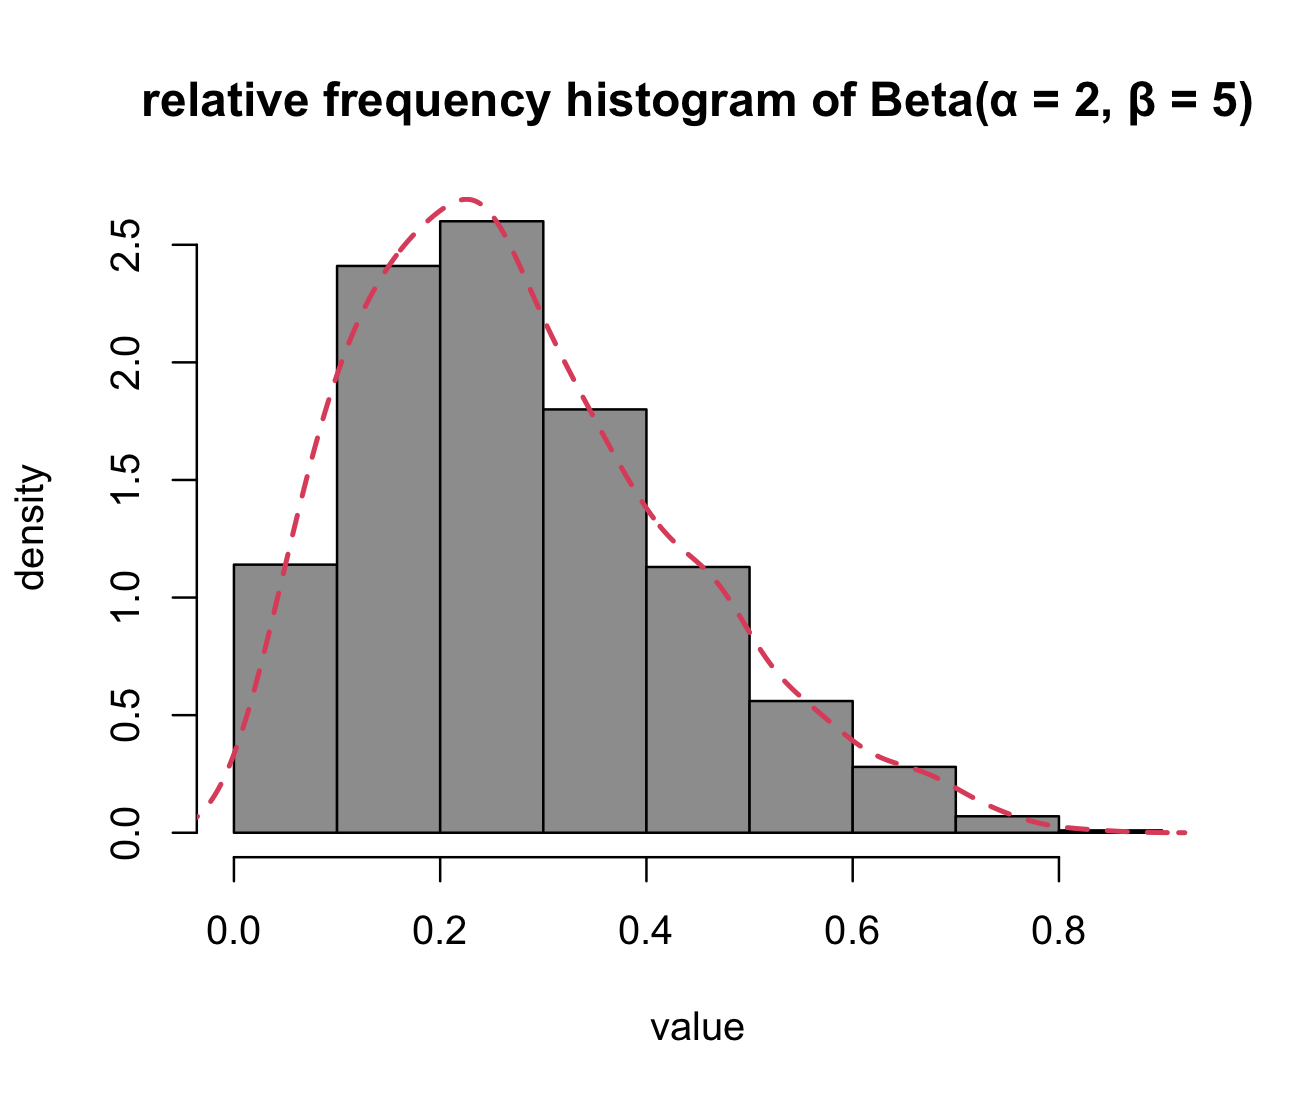
\includegraphics[width=0.45\textwidth]{images/skewed_hist}
        \label{fig:skewed_hist}
    }
    \subfigure[PDF of Skewed Data]{
        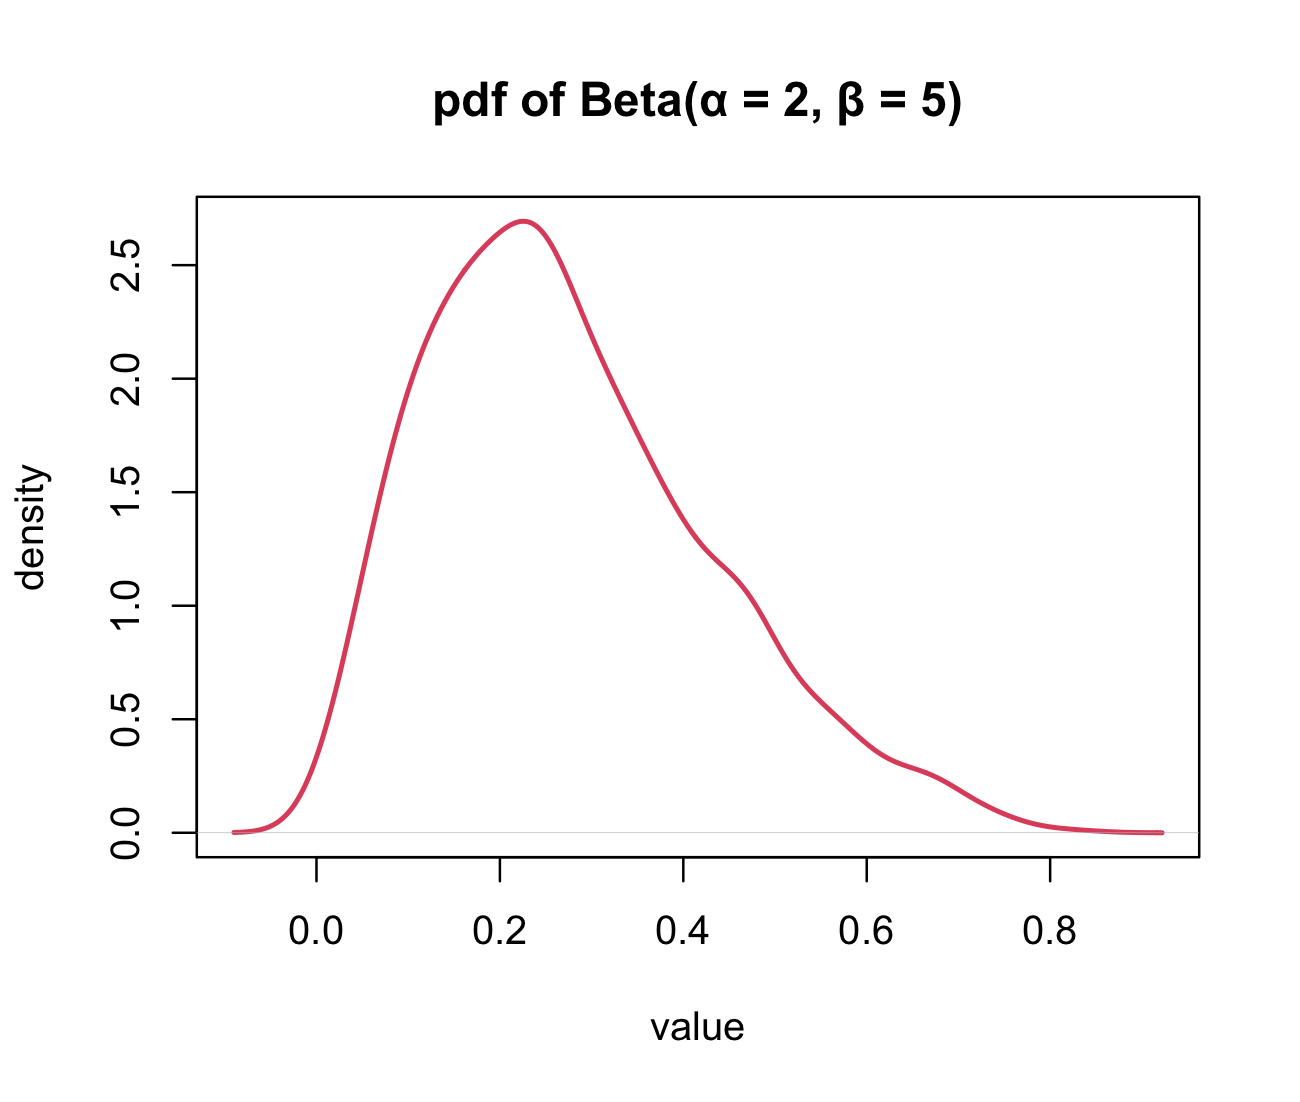
\includegraphics[width=0.45\textwidth]{images/skewed_pdf}
        \label{fig:skewed_pdf}
    }
    \subfigure[Q-Q Plot of Skewed Data]{
        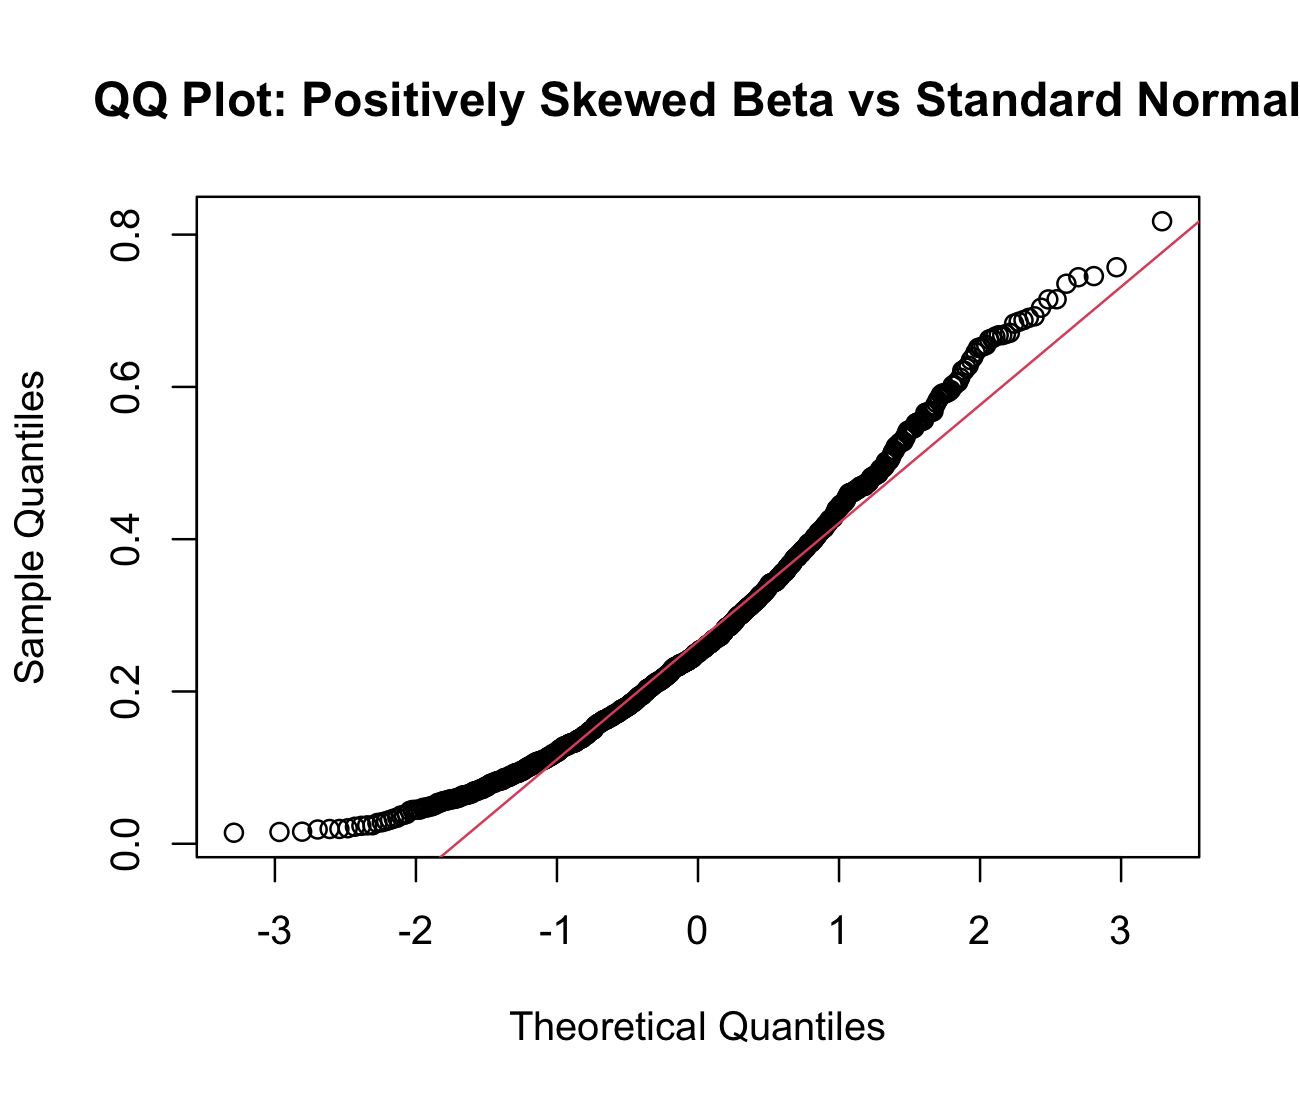
\includegraphics[width=0.45\textwidth]{images/skewed_qq}
        \label{fig:skewed_qq}
    }
    \caption{Q-Q Plot of Skewed Data}
\end{figure}

The QQ plot in Figure \ref{fig:skewed_qq} shows an upward curvature where the points deviate above the line, especially in the tails of the plot. This makes intuitive sense as the lower quantiles are larger in the positive skewed data than in the normal distribution. Furthermore, the right tail also deviates above the line, since in a positively skewed distribution, the right tail is longer and thicker. This leads to higher quantiles at the upper end of the distribution compared to the normal distribution.

The following results suggests that if the data is negatively skewed, for example, $Beta(\alpha = 5, \beta = 2)$, we will see both tails deviate below the line in the QQ plot. $\blacksquare$

\end{document}